
% --------------------------------------------------------------------
% This is a simple Beamer document that uses beamerthemesigma.sty
% Reading the comments should help you create a presentation even if
% you've never used Beamer before.
% --------------------------------------------------------------------
% Set our document class to Beamer
\documentclass[aspectratio=169]{beamer}

% Some packages for nice font encodings in the final PDF
\usepackage[utf8]{inputenc}
\usepackage[T1]{fontenc}

% From Jeff E
\usepackage{algo}

\usepackage{sigmastyle}

% To insert images
\usepackage{graphicx}

% Useful packages from the AMS
\usepackage{amsmath,amssymb,amsthm}

% Package for code highlighting
\usepackage{minted}
\setminted{linenos=true, breaklines=true, breakanywhere=true, style=default}
\usemintedstyle{monokai}

% Set a title
\title{Regular Languages Pt. 2 + Grammars Pt. 1}

% The subtitle is generally where I'd expect you to put the week
% number, thus:
\subtitle{Week 2}
% \texorpdfstring to remove compilation warnings if you have math here

% Whoever worked on the presentation:
\author{Anakin}

% A date, if you'd like.
\date{}

% An institute name, if you're so inclined
% \institute{University of Illinois Urbana-Champaign}

% Use the SIGma theme for this Beamer presentation
\usetheme{sigma}
% --------------------------------------------------------------------
% Begin document
\begin{document}

% Beamer calls each slide a "frame", defined within the environment:
% \begin{frame}
%   <frame content here>
% \end{frame}

% This frame is just the title.
\begin{frame}
\titlepage
\end{frame}

% A frame with the table of contents.
% This frame's title is "Outline".
\begin{frame}{Outline}
  \tableofcontents
\end{frame}

% The frame title is a flag.
\begin{frame}{Updates!}
  % Let's put some real content in this frame:
  \pause
  \begin{itemize}
    \item We want feedback
  \end{itemize}
\end{frame}

\section{Nondeterminism}
\frame{\sectionpage}

\begin{frame}{DFA = \underline{Deterministic} Finite Automata}
    When we talked about DFAs last week, we never really delved into the name \pause
    \begin{itemize}
        \item Automata \pause
        \item Finite \pause
        \item Determinism?
    \end{itemize}
\end{frame}

\begin{frame}{}
    \begin{center}
        \includegraphics[width=\textwidth]{oddDFA.png}
    \end{center}
\end{frame}

\begin{frame}{NFA = \underline{Nondeterministic} Finite Automata}
    What if we removed determinism? \pause
    \begin{center}
        \includegraphics[width=\textwidth]{N1.png}
    \end{center}
\end{frame}

\begin{frame}{}
    \begin{center}
        \includegraphics[width=\textwidth]{N1_multiple_1s.png}
    \end{center}
\end{frame}


\begin{frame}{}
    \begin{center}
        \includegraphics[width=\textwidth]{N1_epsilon.png}
    \end{center}
\end{frame}

\begin{frame}{How I think of NFAs}
    \begin{itemize}
        \item These are confusing at first
        \item Nondeterminism can be thought of in a few ways: \pause
        \begin{itemize}
            \item Guessing \pause
            \item Independent ``processes'' or ``threads'' \pause
            \item When computing over a string, if {\color{sigma@alertred}\textbf{any}} guess is correct, the string is accepted
        \end{itemize}
    \end{itemize}
\end{frame}

% I present to you, some of the hackiest tex known to mankind
\begin{frame}{Computing on an NFA\raisebox{-.6\totalheight}{\includegraphics[scale=0.16]{N1.png}}}
    \begin{center}
        \includegraphics[scale=0.80]{N1_compute/N1_0.png}
    \end{center}
\end{frame}

\begin{frame}{Computing on an NFA\raisebox{-.6\totalheight}{\includegraphics[scale=0.16]{N1.png}}}
    \begin{center}
        \includegraphics[scale=0.80]{N1_compute/N1_1.png}
    \end{center}
\end{frame}

\begin{frame}{Computing on an NFA\raisebox{-.6\totalheight}{\includegraphics[scale=0.16]{N1.png}}}
    \begin{center}
        \includegraphics[scale=0.80]{N1_compute/N1_2.png}
    \end{center}
\end{frame}

\begin{frame}{Computing on an NFA\raisebox{-.6\totalheight}{\includegraphics[scale=0.16]{N1.png}}}
    \begin{center}
        \includegraphics[scale=0.80]{N1_compute/N1_3.png}
    \end{center}
\end{frame}

\begin{frame}{Computing on an NFA\raisebox{-.6\totalheight}{\includegraphics[scale=0.16]{N1.png}}}
    \begin{center}
        \includegraphics[scale=0.80]{N1_compute/N1_4.png}
    \end{center}
\end{frame}

\begin{frame}{Computing on an NFA\raisebox{-.6\totalheight}{\includegraphics[scale=0.16]{N1.png}}}
    \begin{center}
        \includegraphics[scale=0.80]{N1_compute/N1_5.png}
    \end{center}
\end{frame}

% N1_6 is a duplicate of N1_5

\begin{frame}{Computing on an NFA\raisebox{-.6\totalheight}{\includegraphics[scale=0.16]{N1.png}}}
    \begin{center}
        \includegraphics[scale=0.80]{N1_compute/N1_7.png}
    \end{center}
\end{frame}

\begin{frame}{Equivalence}
    \begin{center}
        Turns out NFAs are equivalent to both DFAs and Regex \pause \\[10pt]
        {\Large $\texttt{(0 + 1)}^*\texttt{(101)}\texttt{(0 + 1)}^*\texttt{ + }\texttt{(0 + 1)}^*\texttt{(11)}\texttt{(0 + 1)}^*$}\pause \\[10pt]
        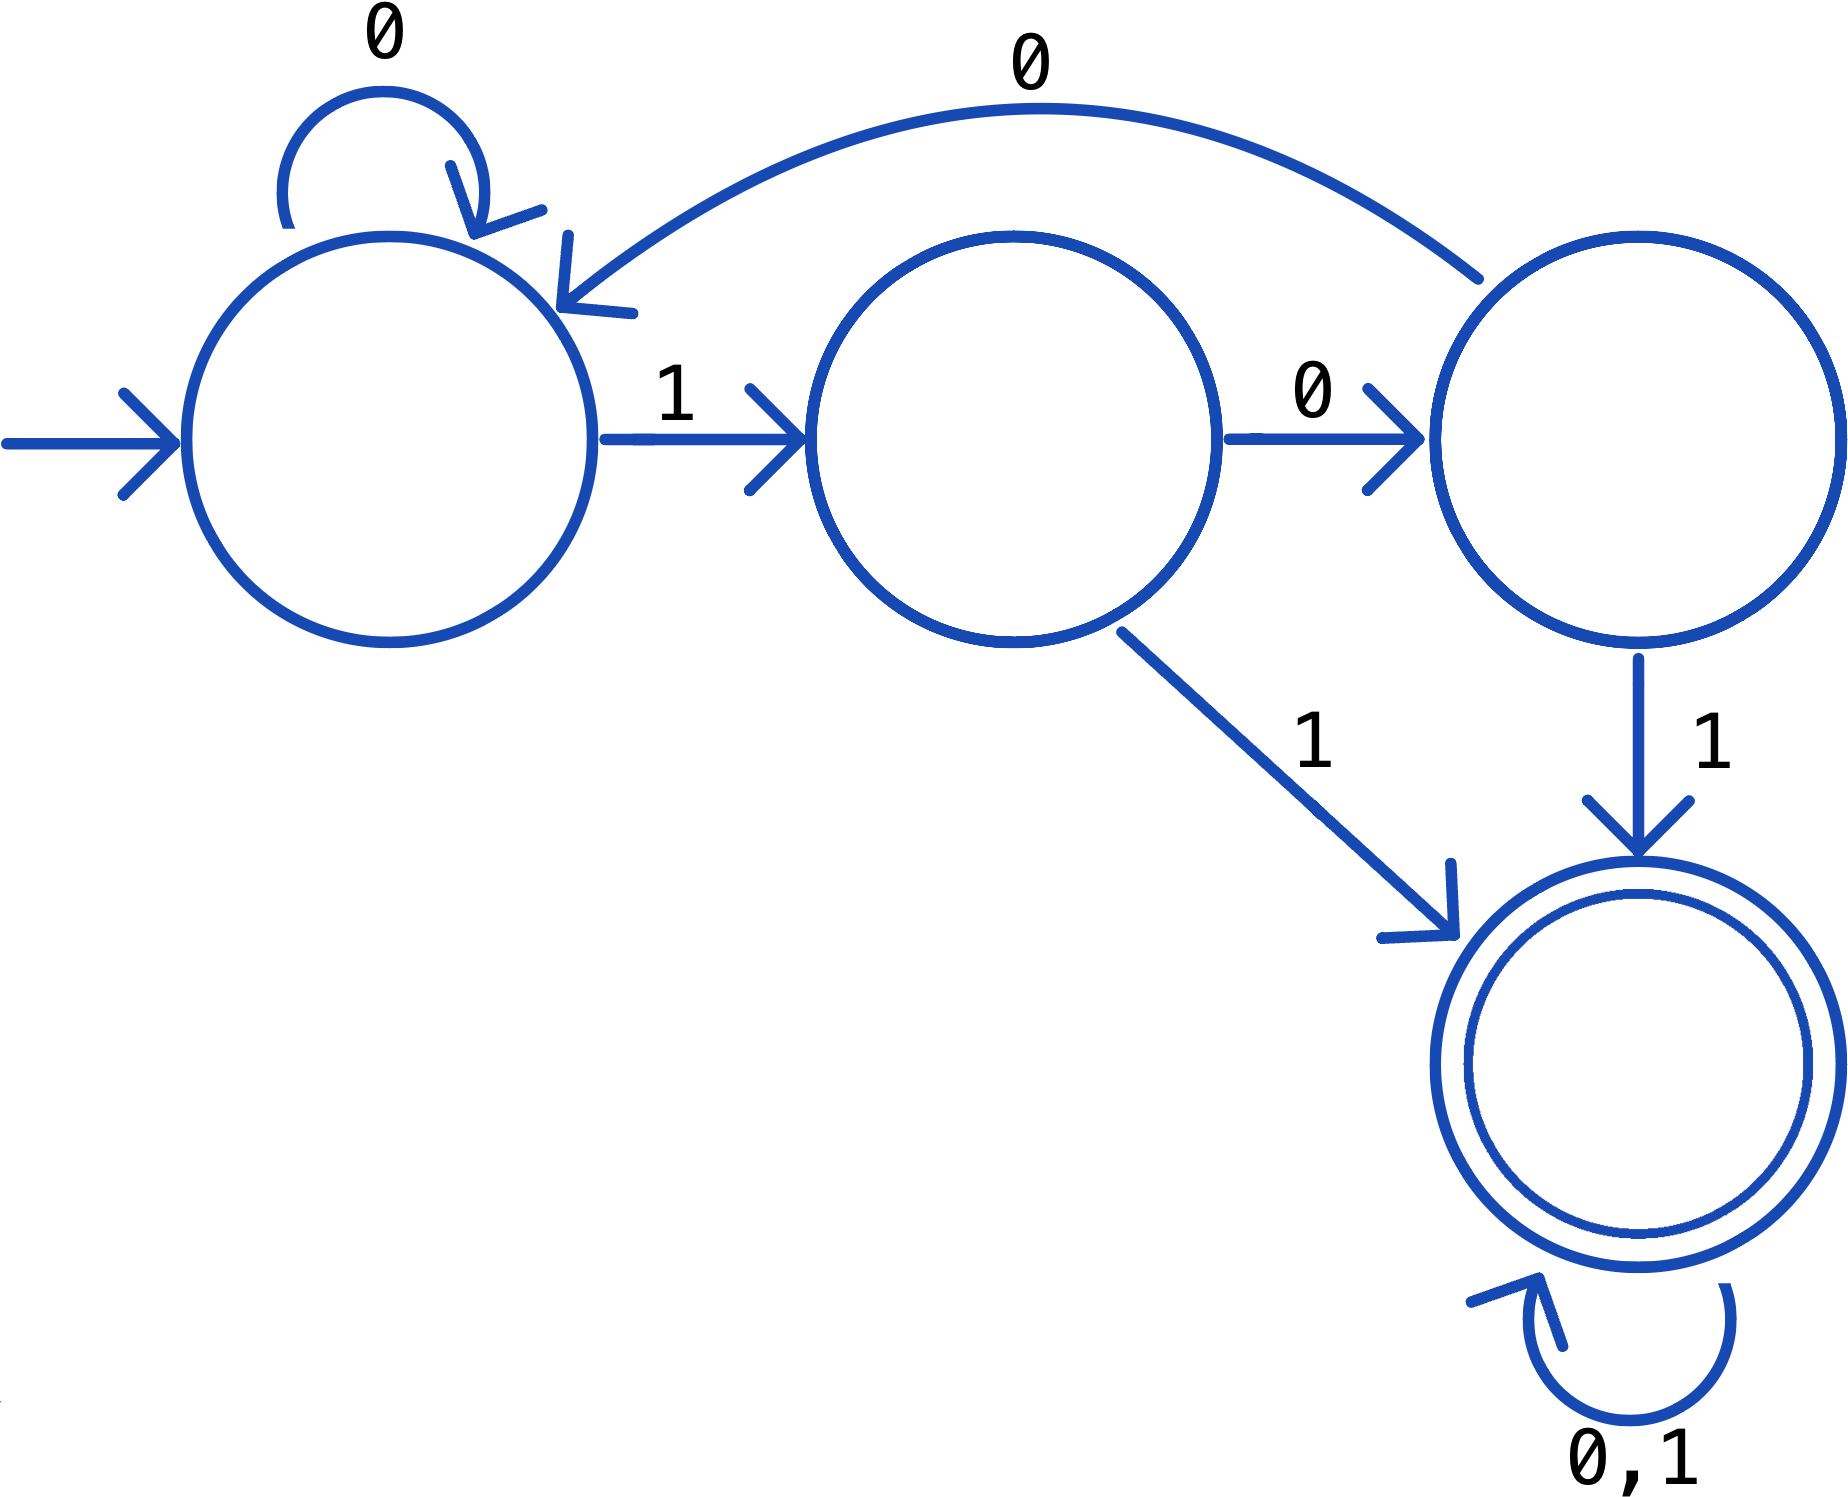
\includegraphics[scale=0.425]{N1_DFA.png}
    \end{center}
\end{frame}

\begin{frame}{NFA \& DFA Equivalence}
    Things aren't always that simple... \pause
    \begin{center}
    \includegraphics[scale=0.15]{N2.png} \pause
    {\Large $$=$$}
    \includegraphics[scale=0.15]{N2_DFA.png}
    \end{center}
    This demonstrates the power of nondeterminism!
\end{frame}


\begin{frame}{}
      \begin{center}
    {\color{sigma@mainblue} \LARGE Questions?}
  \end{center}
\end{frame}

\begin{frame}{Questions!}
    
    Take the following description for a language and come up with a regex, NFA, and DFA for it
    $$
    ``w \textrm{ contains an even number of } \texttt{0} \textrm{'s, or contains exactly two } \texttt{1} \textrm{'s}"
    $$
    
\end{frame}

% Start a section: *sections* (subsections, etc.) are what show up in the TOC.
\section{Context Free Grammars}
% Section pages can be printed thus:
\frame{\sectionpage}
% There's a way to automate this, see:
% https://tex.stackexchange.com/questions/178800/creating-sections-each-with-title-pages-in-beamers-slides/178803

\begin{frame}{Recursion}
    \begin{itemize}
        \item DFAs / NFAs give us \textbf{iteration} and \textbf{state} \pause
        \item Pure \textbf{recursion} is not emulated by DFAs / NFAs
    \end{itemize}
\end{frame}

\begin{frame}{Context Free Grammars}
    {
    \LARGE
    \vspace{20pt}
    \begin{align*}
        A ~&\to~ \texttt{0}A\texttt{1} \\
        A ~&\to~ B                     \\
        B ~&\to~ \varepsilon           \\
    \end{align*}
    }
\end{frame}

\begin{frame}{Context Free Grammars}
    {
    \LARGE
    \vspace{20pt}
    \begin{align*}
        {\color{sigma@alertred}A} ~&\to~ \texttt{0}A\texttt{1} \\
        {\color{sigma@alertred}A} ~&\to~ B                     \\
        {\color{sigma@alertred}B} ~&\to~ \varepsilon           \\
    \end{align*}
    }
\end{frame}

\begin{frame}{Context Free Grammars}
    {
    \LARGE
    \vspace{20pt}
    \begin{align*}
        A ~&{\color{sigma@alertred}\to}~ \texttt{0}A\texttt{1} \\
        A ~&{\color{sigma@alertred}\to}~ B                     \\
        B ~&{\color{sigma@alertred}\to}~ \varepsilon           \\
    \end{align*}
    }
\end{frame}

\begin{frame}{Context Free Grammars}
    {
    \LARGE
    \vspace{20pt}
    \begin{align*}
        A ~&\to~ \texttt{0}{\color{sigma@alertred}A}\texttt{1} \\
        A ~&\to~ {\color{sigma@alertred}B}                     \\
        B ~&\to~ \varepsilon           \\
    \end{align*}
    }
\end{frame}

\begin{frame}{Context Free Grammars}
    {
    \LARGE
    \vspace{20pt}
    \begin{align*}
        A ~&\to~ {\color{sigma@alertred}\texttt{0}}A{\color{sigma@alertred}\texttt{1}} \\
        A ~&\to~ B                      \\
        B ~&\to~ {\color{sigma@alertred}\varepsilon}           \\
    \end{align*}
    }
\end{frame}

\begin{frame}{Context Free Grammars}
    {
    \LARGE
    \vspace{20pt}
    \begin{align*}
        A ~&\to~ \texttt{0}A\texttt{1} \\
        A ~&\to~ B                     \\
        B ~&\to~ \varepsilon           \\
    \end{align*}
    }
\end{frame}

\begin{frame}{Context Free Grammars}
    {
    \LARGE
    \vspace{30pt}
    \begin{align*}
        A ~&\to~ \texttt{0}A\texttt{1} ~{\color{sigma@alertred}|}~ B \\
        B ~&\to~ \varepsilon           \\
    \end{align*}
    }
\end{frame}

\begin{frame}{Context Free Grammars}
    {
    \LARGE
    \vspace{40pt}
    \begin{align*}
        A ~&\to~ \texttt{0}A\texttt{1} ~|~ \varepsilon \\
    \end{align*}
    }
\end{frame}

\begin{frame}{Is a string in a CFG?}
    \begin{center}
        \includegraphics[scale=0.33]{CFG_tree.png}
    \end{center}
\end{frame}

\begin{frame}{Derivations}
    $$
        A \pause\Rightarrow \texttt{0}A\texttt{1} \pause\Rightarrow \texttt{00}A\texttt{11} \pause\Rightarrow \texttt{000}A\texttt{111} \pause\Rightarrow \texttt{000}B\texttt{111} \pause\Rightarrow \texttt{000}\varepsilon\texttt{111} \pause\Rightarrow \texttt{000}\texttt{111}
    $$
\end{frame}

\begin{frame}{Equivalence with Regular Languages?}
    \begin{itemize}
        \item CFGs define a language \pause
        \item A natural question is ``are these languages also regular languages?'' \pause
        \begin{itemize}
            \item Turns out the answer is no! \pause
            \item Every regular language is context free \pause
            \item The opposite is not true. Consider $\Set{\texttt{0}^n\texttt{1}^n | n \geq 0}$
        \end{itemize}
    \end{itemize}
\end{frame}

\begin{frame}{}
      \begin{center}
    {\color{sigma@mainblue} \LARGE Questions?}
  \end{center}
\end{frame}

\begin{frame}{Questions!}

    \begin{itemize}
        \item Come up with a CFG to match strings with twice as many \texttt{a}'s as \texttt{b}'s
        \item Come up with a CFG to match strings with balanced parentheses, brackets, and braces: \texttt{(), [], \{\}}.
    \end{itemize}
    
\end{frame}

\font\eightss=cmssq8
\font\eightssi=cmssqi8
\newcommand\quoteAuthorDate[3]{\begingroup
  \baselineskip 10pt
  \parfillskip 0pt
  \interlinepenalty 10000 % not needed in example
  \leftskip 0pt plus 40pc minus \parindent
  \let\rm=\eightss
  \let\sl=\eightssi
  \everypar{\sl}#1\par
  \nobreak\smallskip
  \noindent\rm--- #2\unskip\enspace(#3)\par
  \endgroup}

\begin{frame}{Goodbye}
    \centering
    \quoteAuthorDate{``You may not instantly see why I bring the subject up, but that is because my mind works so phenomenally fast, and I am at a rough estimate thirty billion times more intelligent than you. Let me give you an example. Think of a number, any number.'' \par``Er, five,'' said the mattress.\par``Wrong,'' said Marvin. ``You see?''}{DOUGLAS ADAMS}{1979}
\end{frame}


\end{document}